
\documentclass[12pt]{article}
\usepackage[utf8]{inputenc}
\usepackage{minted}
\usepackage{graphicx} % Allows you to insert figures
\usepackage{amsmath} % Allows you to do equations
\usepackage{fancyhdr} % Formats the header
\usepackage{geometry} % Formats the paper size, orientation, and margins
\linespread{1.25} % about 1.5 spacing in Word
\setlength{\parindent}{0pt} % no paragraph indents
\setlength{\parskip}{1em} % paragraphs separated by one line
\usepackage[format=plain,
            font=it]{caption} % Italicizes figure captions
\usepackage[english]{babel}
\usepackage{csquotes}
\renewcommand{\headrulewidth}{0pt}
\geometry{letterpaper, portrait, margin=1in}
\setlength{\headheight}{14.49998pt}
\geometry{a4paper, left=20mm, right=20mm, top=20mm, bottom=20mm}

\newcommand\titleofdoc{\LARGE{\textbf{Assignment-10: Linear and Circular Convolution}}}
\newcommand\GroupName{EE20B136}

\begin{document}
\begin{titlepage}
   \begin{center}
        \vspace*{4cm} % Adjust spacings to ensure the title page is generally filled with text

        \Huge{\titleofdoc} 

        \vspace{3 cm}
        \Large{Syam SriBalaji T}
       
        \vspace{0.25cm}
        \large{EE20B136}
       
        \vspace{3 cm}
        \Large{May 14, 2022}
        
        \vspace{0.25 cm}
        \Large{EE2703 :Jan-May 2022}
       

       \vfill
    \end{center}
\end{titlepage}

\setcounter{page}{2}
\pagestyle{fancy}
\fancyhf{}
\rhead{\thepage}

\section*{\textbf{Introduction:}}
In this assignment, we will be working on 
\begin{itemize}
  \item Linear Convolution
  \item Circular Convolution
  \item Circular Convolution using Linear Convolution
  \item Correlation output of Zadoff-Chu sequences
\end{itemize}

\section*{Magnitude and Phase plot of the given filter:}

Firstly we read the file \textit{'h.csv'} which contains coefficients for an FIR filter. Now we use \textit{'sig.freqs()'} from scipy library to convert given values from time domain to frequency domain.

\begin{figure}[h!]
\centering
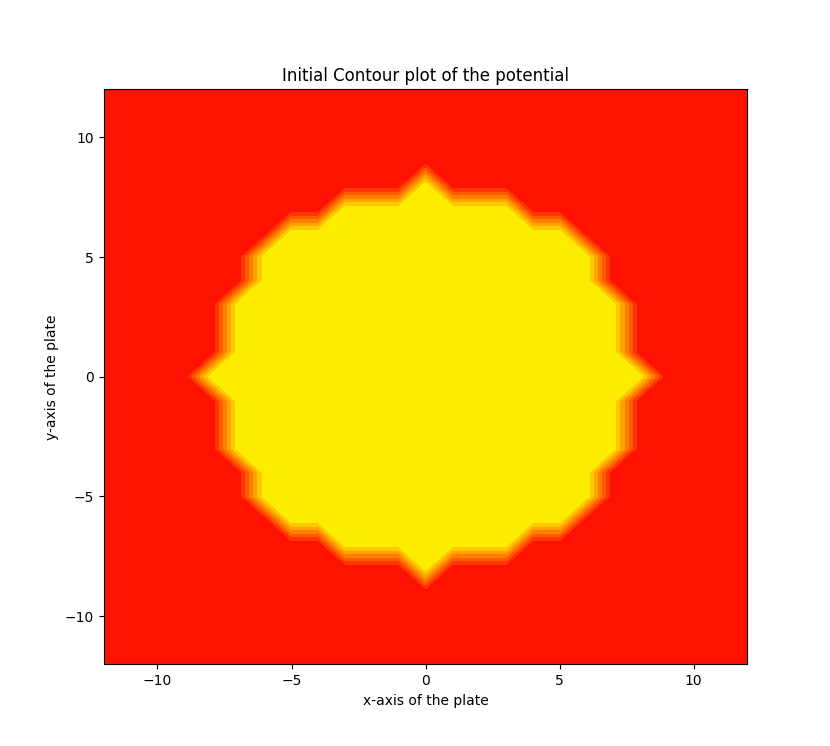
\includegraphics[height=11cm]{Figure_1.png}
\end{figure}

\newpage
\section*{Graph of {\boldmath $x = cos(0.2\pi n) + cos(0.85 \pi n)$}:}

Here is the normal plot of $cos(0.2\pi n) + cos(0.85 \pi n)$ , we using \textit{'linspace()'} to create the points in x-axis.
\begin{figure}[h!]
\centering
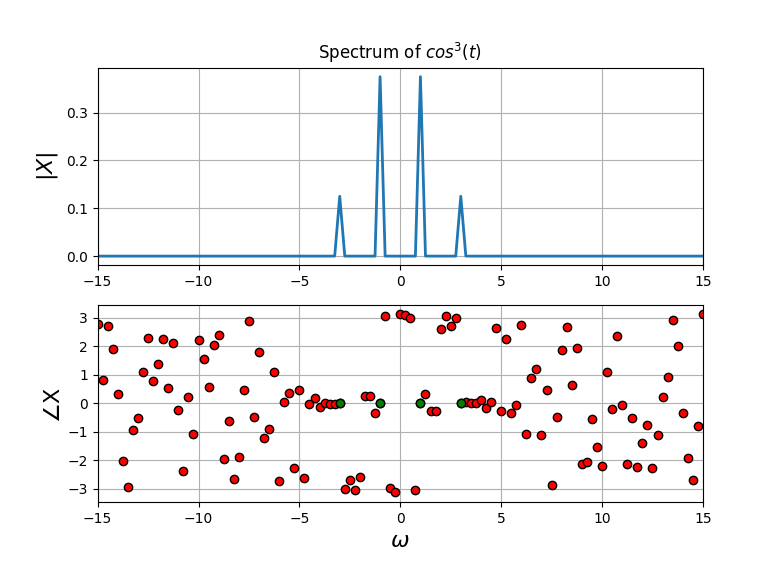
\includegraphics[height=7cm]{Figure_2.png}
\end{figure}
\section*{Linear convolution:}
Linear convolution for a sequence is-
\begin{equation}
    y[n] = \sum_{k=0}^{n-1} x[n-k]h[k]
\end{equation}

While in Python will be simply using \textit{'convolve()'} from numpy library and solve linear convolution of x which we got from previous question.
\begin{figure}[h!]
\centering
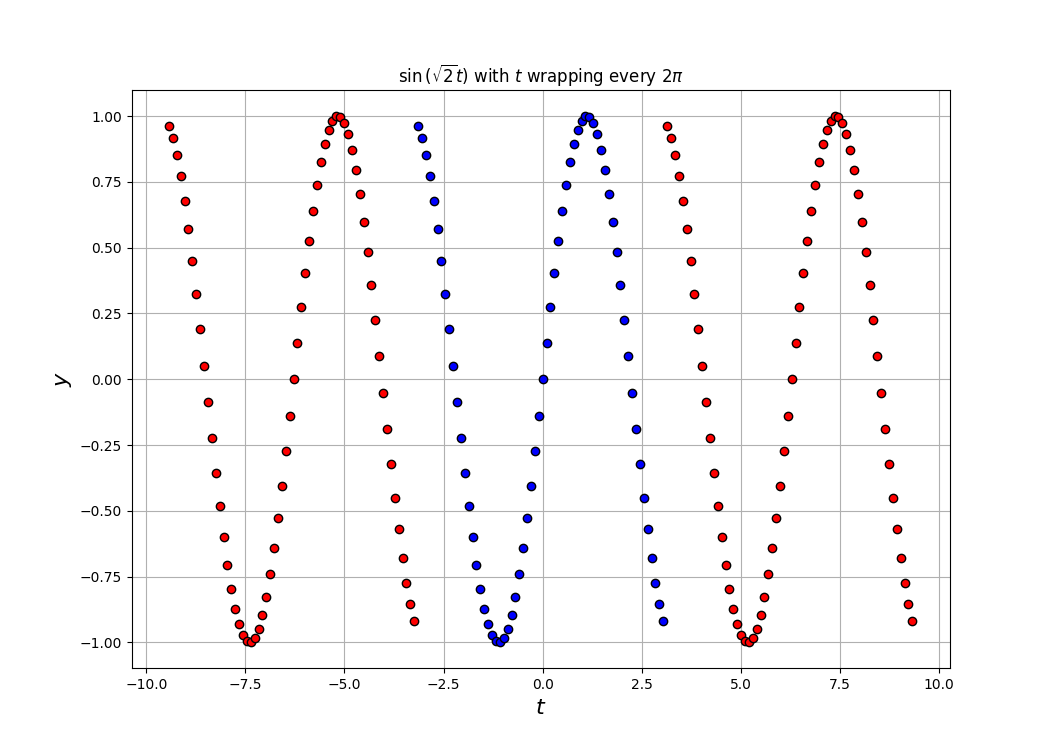
\includegraphics[height=7cm]{Figure_3.png}
\label{fig:exemplo}
\end{figure}

\newpage
\section*{Circular convolution: }

The DFT supporting convolution is given by-

\begin{equation}
  \begin{aligned}
    \tilde{x}[n] = \frac{1}{N} \times \sum_{k=0}^{N-1} \tilde{X}[k]e^{j(\frac{2\pi}{N})kn}\\
    \tilde{X}[k]= \sum_{k=0}^{N-1} \tilde{n}[n]e^{-j(\frac{2\pi}{N})kn}
  \end{aligned}
\end{equation}

here $\tilde{x}$ refers that the sequence of N values are extended into infinite periodic sequence.

  \begin{equation}
    \tilde{x}[n]=
    \begin{cases}
      x[n]    &   0 \le n < N\\
      x[n-N]  &   N \le n < 2N\\
      x[n+N]  & -N \le n < 0
    \end{cases}
  \end{equation}

Thus, the circular convolution is given by-

\begin{equation}
  \begin{aligned}
    \tilde{y}[n] = \sum_{m=0}^{N-1} \tilde{x}[n-m]\tilde{h}[k]\\
    \tilde{y}[n] = \sum_{m=0}^{N-1} x[(n-m) ~\textit{modulo}~ N]~h[m]
  \end{aligned}
\end{equation}

The length of the output y[n] is expected to be len(x)+len(h)-1. The input x[n] and transfer sequence h[n] are done with zero padding because the number of frequency in DFT and time domain are same. So now in Python we simply use \textit{'concatenate'} from numpy library. to obtain circular convolution.

\begin{figure}[h!]
\centering
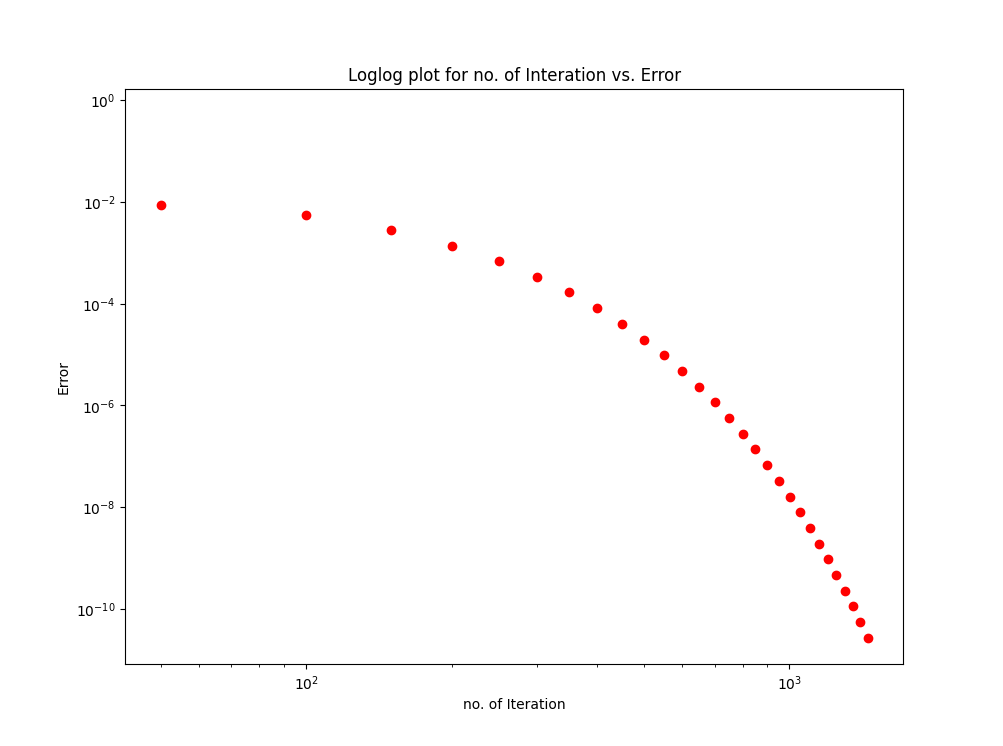
\includegraphics[height=6.5cm]{Figure_4.png}
\label{fig:exemplo}
\end{figure}


\newpage
\section*{Linear convolution using Circular convolution:}

For this method, the following procedure is to be followed-\\\\
1. When h[n] fits in $2^m$ window so it is zero padded\\
2. x[n] is broken into $2^m$ divisions\\
3. Appropriate padding is added to each DFTs\\
4. Bring back all the outputs and combining it\\
So we process it by-
\begin{minted}{python}
def Circ_conv(x,h):
    P1 = len(h)
    n_ = int(ceil(log2(P1)))
    h_ = concatenate((h,zeros(int(2**n_)-P1)))
    P2 = len(h_)
    n1 = int(ceil(len(x)/2**n_))
    x_ = concatenate((x,zeros(n1*(int(2**n_))-len(x))))
    y = zeros(len(x_)+len(h_)-1)
    for i in range(n1):
        temp = concatenate((x_[i*P2:(i+1)*P2],zeros(P2-1)))
        y[i*P2:(i+1)*P2+P2-1] += np.fft.ifft(np.fft.fft(temp) * np.fft.fft( concatenate
        ( (h_,zeros(len(temp)-len(h_))) ))).real
    return y
\end{minted}

From that, we plot the Circular convolution using Linear convolution of x. And also we can note that this is similar to the graph which we got earlier. 

\begin{figure}[h!]
\centering
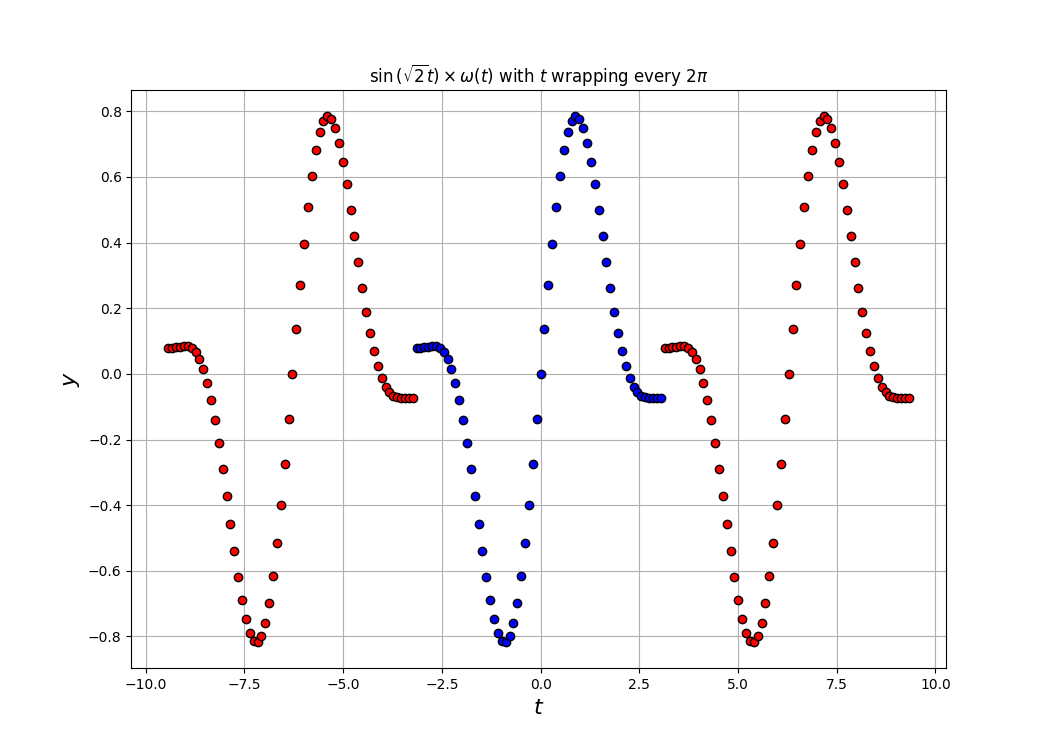
\includegraphics[height=8cm]{Figure_5.png}
\label{fig:exemplo}
\end{figure}
 
\newpage
\section*{Correlation output plot of Zadoff-Chu sequences:}

The properties of Zadoff-Chu sequence are-\\\\
1. It is a complex and constant amplitude sequence.\\
2. Auto correlation of it's sequence with a cyclically shifted version of itself is zero.\\
3. Correlation of it's sequence with the delayed version of itself will give a peak at that delay.\\

Thus, after Auto-correlating Zandoff Chu sequence, we get-

\begin{figure}[h!]
\centering
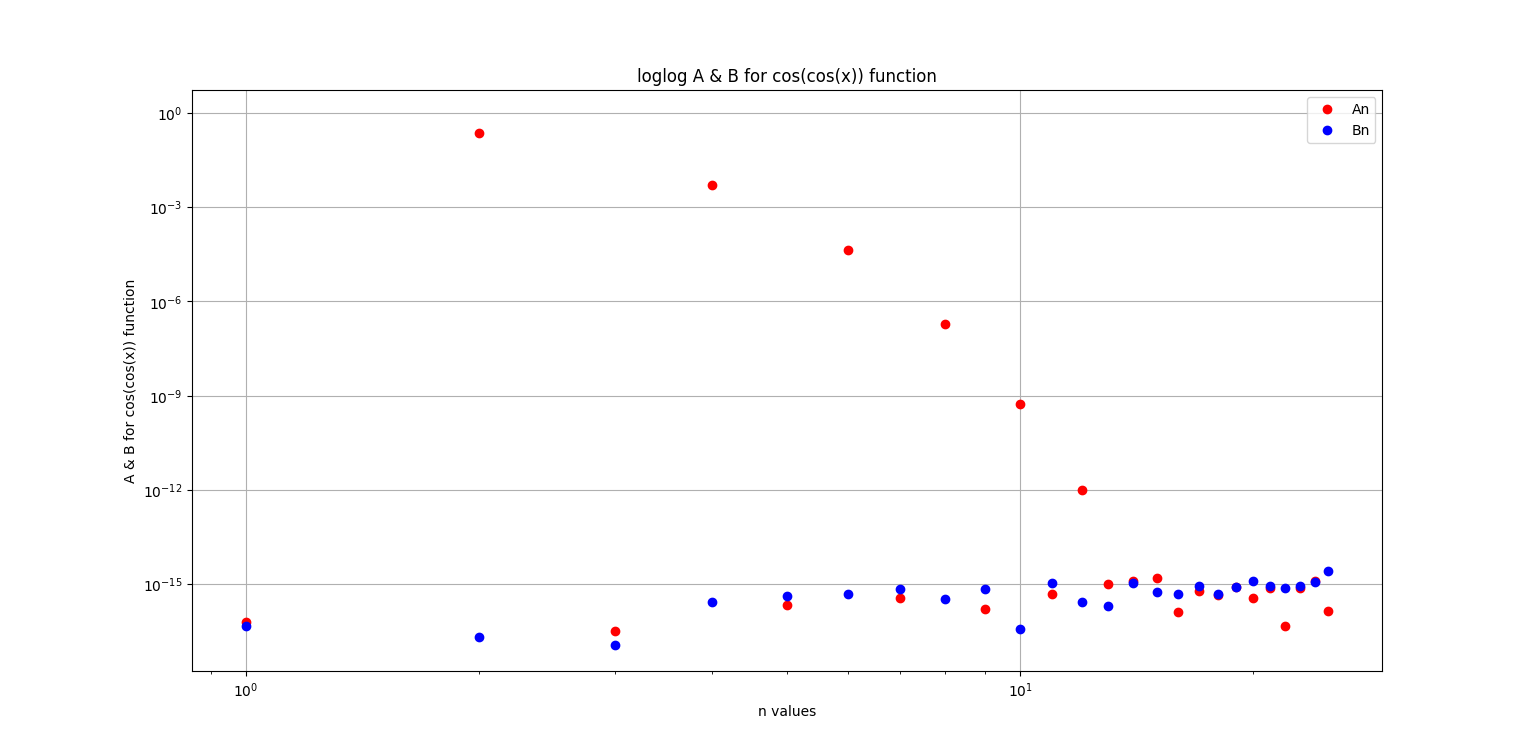
\includegraphics[height=8cm]{Figure_6.png}
\label{fig:exemplo}
\end{figure}
And we can view that the peak is present at 5.

\section*{Conclusion:}
Thus, in this assignment we understood that we can do Linear convolution, Circular convolution, Correlation for various different kinds of input signals in Python easily. 
\begin{center} 
\textbf{Thank you!}
\end{center} 
\end{document}
